\documentclass{article}
\usepackage[margin=0.5in]{geometry}
\usepackage{color}
\usepackage{setspace}
\usepackage{graphicx}
\setlength{\intextsep}{0.5cm}
\usepackage{textcomp}
\usepackage{setspace}
\usepackage{palatino}
\usepackage{hyperref}
\usepackage{fancyvrb}

\hypersetup{
	colorlinks=true, %set true if you want colored links
	linktoc=all,     %set to all if you want both sections and subsections linked
	linkcolor=blue,  %choose some color if you want links to stand out
	urlcolor=blue
}


\begin{document}

\title{Introduction to Python \\ Installation Instructions for Mac}
\author{Stephanie Spielman \\ \footnotesize{Email: stephanie.spielman@gmail.com}}
\date{}
\maketitle{}

Note that these instructions are guaranteed work for Mac OS Mavericks and Yosemite. I'm reasonably sure that these instructions will be fine for early OS versions, but if you encounter difficulty please to do not hesitate to email Stephanie! The instructions below were adapted from \href{http://sjspielman.org/configure_yosemite_biocomputing/}
{http://sjspielman.org/configure\_yosemite\_biocomputing/}.


\begin{enumerate}
	\item If you do not have it installed already, download XCode from the Mac App Store.
	
	\item You'll need to have a text editor you feel comfortable using. Mac comes with a native text editor, called TextEdit, but for the purposes of programming, it's pretty bad, so \emph{do not use it when coding}. XCode also comes with it's own text editor, called XCode, which you are more than welcome to use. Personally, I use TextWrangler, which is freely available for download here: \\ \href{http://www.barebones.com/products/textwrangler/download.html}{http://www.barebones.com/products/textwrangler/download.html}. I highly recommend getting TextWrangler!!
	
	\item Although Mac does come with its own version of Python, this distribution has a tendency to play poorly with certain Python libraries. Therefore, we'll be using the Python distribution from \href{https://brew.sh}{Homebrew}. Homebrew is a general Mac package manager -- it's amazingly useful for downloading and managing software! 
	\\\\
	To install Homebrew, open a \textbf{Terminal} window. The terminal, or command line, is the application used to interact with your computer, so you'll be using it all the time. I recommend keeping Terminal in your Dock for convenience. To open Terminal, either type "Terminal" into Spotlight, or open directly from Applications $\rightarrow$ Utilities. Once you've opened Terminal, enter the following command:
	\begin{Verbatim}[fontsize=\small,xleftmargin=-2.5cm,commandchars=+\[\]]
		+textbf[sudo ruby -e "$(curl -fsSL https://raw.githubusercontent.com/Homebrew/install/master/install)"]
	\end{Verbatim}
	After you press enter, you will be prompted for your password (the same one you use when you turn on/sign in to your computer). Type in your password, and then press enter again. You'll notice that keystrokes will \emph{not} appear in the Terminal - this is ok!!
	
	\item Now that Homebrew has been installed, we can use it to install Python. Enter these commands, in this order, into Terminal: 
	\begin{Verbatim}[fontsize=\small,xleftmargin=-0.95cm,commandchars=+\[\]]
	+textbf[brew install readline --universal]
	+textbf[brew install python]
	\end{Verbatim}
	
	If, after typing either of these commands, you receive an error indicating that you do not have \emph{Permissions} to install, then re-enter the command with the word \textbf{\texttt{sudo}} in front (you may be prompted for your password again), e.g.\ :
	\begin{Verbatim}[fontsize=\small,xleftmargin=-0.95cm,commandchars=+\[\]]
	+textbf[sudo brew install readline --universal]
	+textbf[sudo brew install python]
	\end{Verbatim}
	
	\item Finally, we'll install a few useful Python packages. For this, we'll use \textbf{\texttt{pip}}, a Python package manager. Homebrew's Python installation actually comes with pip, so you can simply start using it. Enter the following commands to (1) update pip (usually needed) and (2) install iPython.
	
	\begin{Verbatim}[fontsize=\small,xleftmargin=-0.95cm,commandchars=+\[\]]
	+textbf[pip install --upgrade pip]
	+textbf[pip install ipython]
	\end{Verbatim}

\end{enumerate}

\noindent To confirm that everything worked well, type \textbf{\texttt{ipython}} into your Terminal. This should launch an iPython session, which looks something like this:

\begin{center}
	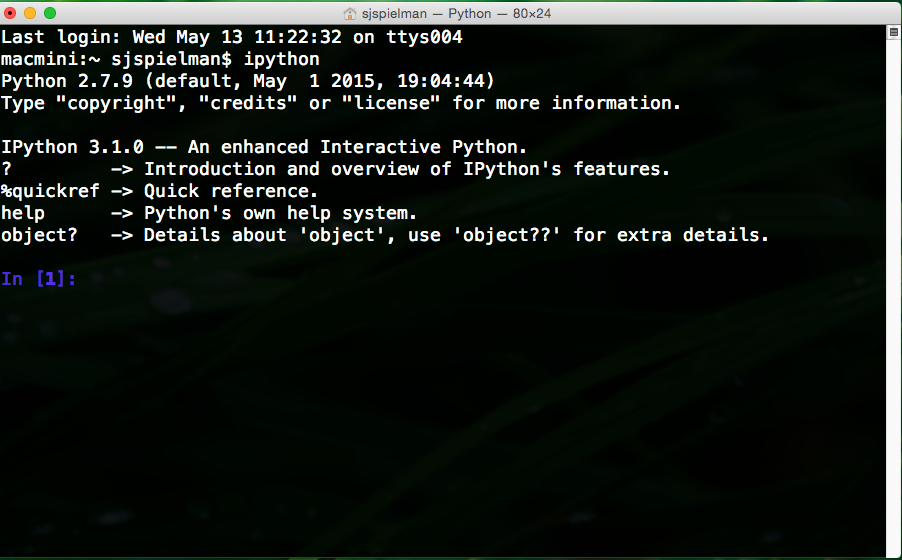
\includegraphics[width=3.75in]{ipython_session.png}
\end{center}	


To exit iPython, press \textbf{\texttt{ctrl+d}}, and type y (to indicate "yes", you really do want to exit). Exit the current Terminal session by typing \textbf{\texttt{exit}}. You're all done, now!

\end{document}
